% Section content template for individual Educative lessons
% This file contains the actual content for a specific section
% Generated from Educative API section content

% Section: Interview Tips
% Section ID: 6310221117128704
% Section Slug: interview-tips
% Generated: 2025-12-14T14:24:59.445760

% \vspace{-1.0\baselineskip}
\noindent
\begin{minipage}[t]{0.48\textwidth}\vspace{0pt}
Substantial preparation is necessary to increase our chances of getting the job we've applied for. Depending on a candidate's seniority and proficiency, different candidates need different amounts of times for interview preparation. For an average candidate, three to four months might be required to prepare for an object-oriented design interview.
\end{minipage}
\hfill
\begin{minipage}[t]{0.48\textwidth}\vspace{0pt}
\centering

\includegraphics[width=0.5\textwidth]{Images/chapter_28/section_6310221117128704/6316688662593536.png}
\end{minipage}

\subsection{Mock interviews}\label{kE7i7_GLMarfVW9aa2GMB}
\\
\href{https://www.educative.io/mock-interview}{\textbf{Mock interviews}} are a great way to prepare for the object-oriented design interviews. They involve pairing up with a friend and allowing them to ask questions. If a friend is not available, another strategy is to record ourselves and play the role of both the interviewer and interviewee. With this approach, we can critique ourselves or ask a knowledgeable friend for feedback.

% \vspace{-1.0\baselineskip}
\noindent
\begin{minipage}[t]{0.48\textwidth}\vspace{0pt}
The interviewer has probably asked many candidates the same question. Reproducing a run-of-the-mill design might not impress the interviewer.
\\
At the same time, an interview can be a stressful situation. Having a plan to tackle the problem might be a good strategy. Depending on the candidate, there can be multiple strategies to address a design problem. We suggest the following technique:
\end{minipage}
\hfill
\begin{minipage}[t]{0.48\textwidth}\vspace{0pt}
\centering

\includegraphics[width=0.5\textwidth]{Images/chapter_28/section_6310221117128704/6750202833928192.png}
\end{minipage}

\subsection{Strategize, divide, and conquer}\label{tp61qQJYV1eYr1PwSBOLB}
\\
We recommend including the following activities somewhere in the interview:

\begin{figure}[htbp]
 \centering
 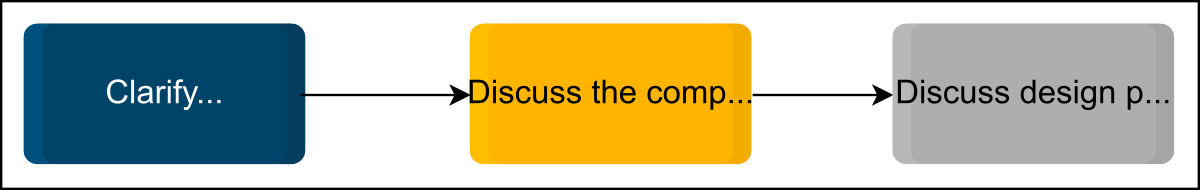
\includegraphics[width=0.5\textwidth]{Images/chapter_28/section_6310221117128704/6289731518464000.png}
 \caption{Activities to include in the interview}
\end{figure}

\subsubsection{Clarify requirements}\label{Q92myEvdH2sSwCRN7JmV9-2}
\\
The interviewer provides you with a design problem and a set of requirements. As an interview candidate, you need to ask the interviewer questions from to clarify the requirements and narrow down the scope of the problem so that it can be solved within 30--40 minutes. Clearly defined requirements can help visualize the design solution.

\subsubsection{Discuss the components}\label{nAlmeN6Yv8xV8qLTDjLwl}
\\
You need to start solving the problem by identifying the components required for the design. The nouns in the requirements can translate as objects in our system. However, the verbs can be categorized as the methods or actions these objects can perform. As you categorize the requirements in this manner, it becomes easier to see the individual components. You should make sure to discuss your approach with the interviewer clearly so that they can understand your thought process.

\subsubsection{Discuss design patterns}\label{s7jRUvbNig7K0fC0W7FGT}
\\
The best solution is one that is easily maintainable and extendable. Interviewers often ask follow-up questions about what design patterns can be used to improve the quality of the proposed solution. You should be well-versed in some of the most commonly occurring design patterns. It leaves a great impression on the interviewer if you can correctly use design patterns in the appropriate components.

\subsection{What not to do in an interview}\label{En2x4v-1jo0BtN8rx43-4}

% \vspace{-1.0\baselineskip}
\noindent
\begin{minipage}[t]{0.48\textwidth}\vspace{0pt}
Here are a few things that you should avoid in an object-oriented design interview: - Don't start building without a plan. - Don't work in silence. It is encouraged to think out loud during the interview. - Don't code the implementation of the system unless specifically asked. You only need to define your classes and methods. - If you don't know something, don't pretend to know it.
\end{minipage}
\hfill
\begin{minipage}[t]{0.48\textwidth}\vspace{0pt}
\centering
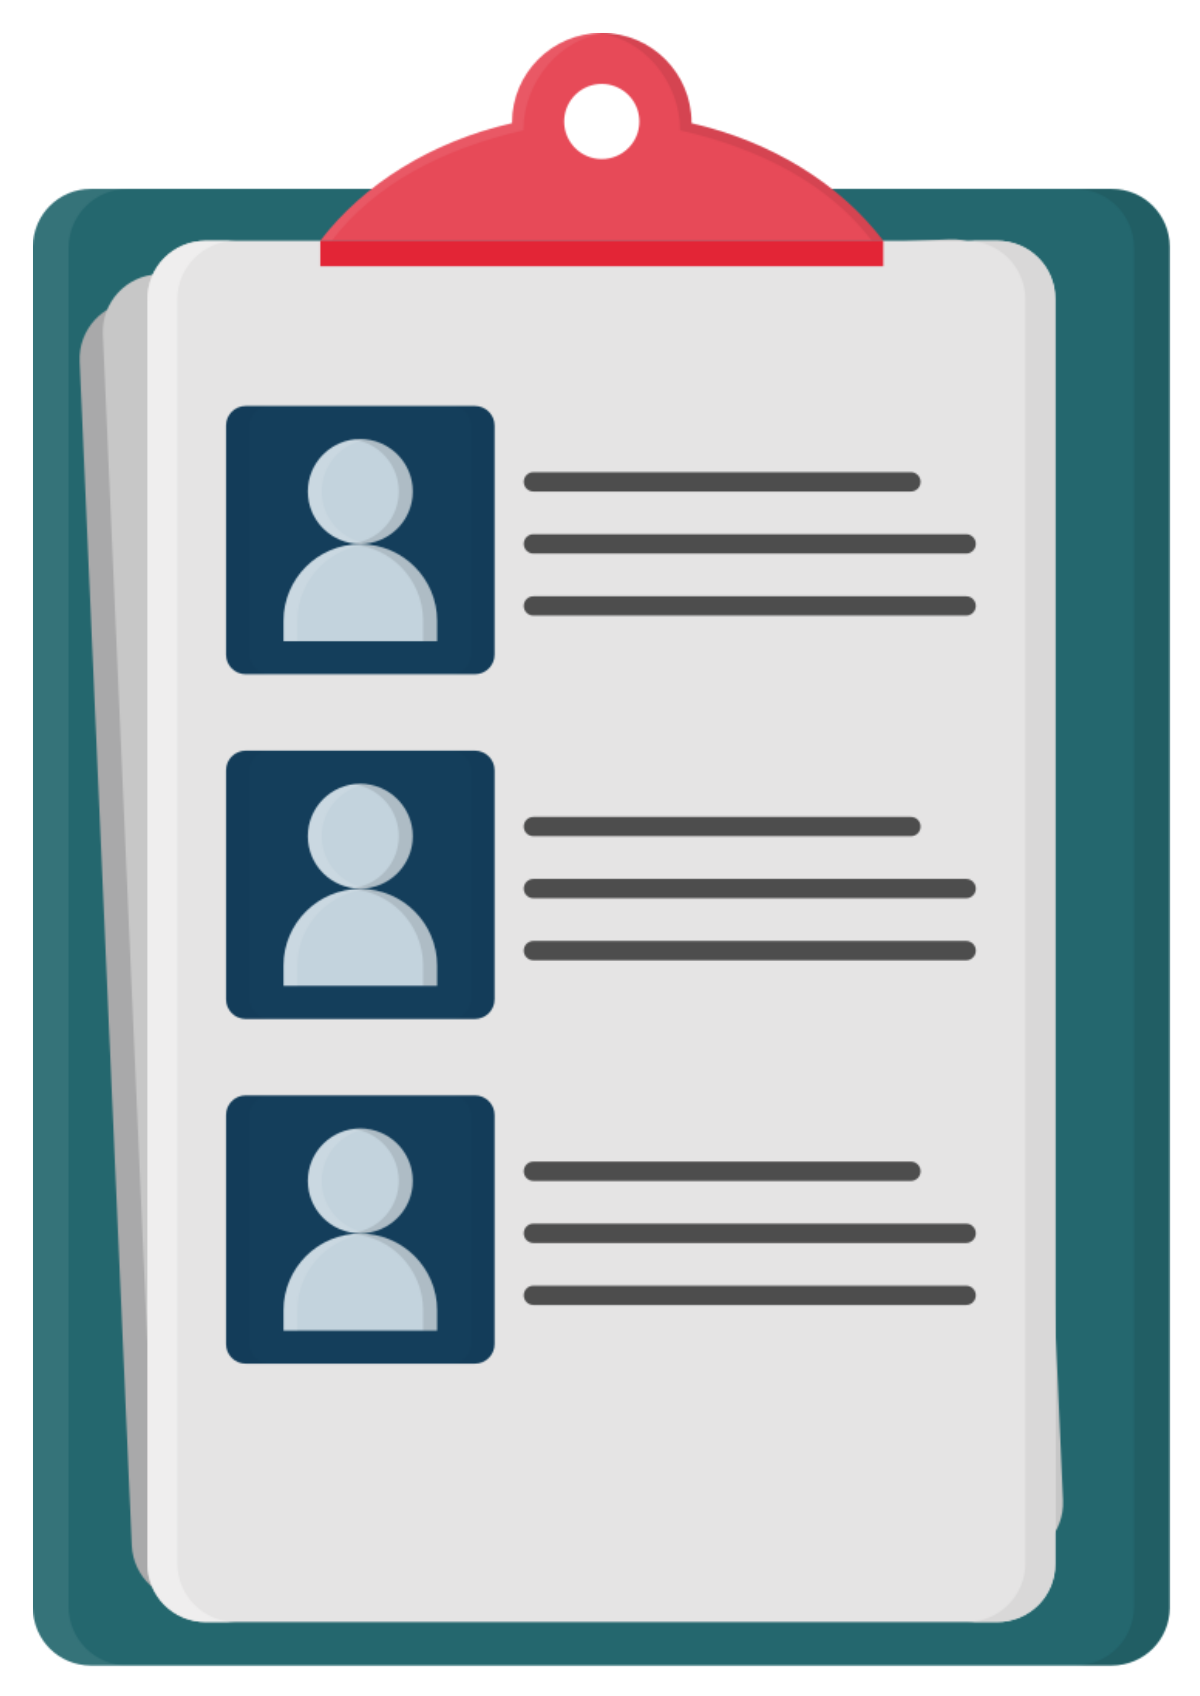
\includegraphics[width=0.25\textwidth]{Images/chapter_28/section_6310221117128704/5243652379901952.png}
\end{minipage}

\begin{quote}
\textbf{Note:} If an interviewer asks you about a design problem you haven't heard of, you should just be honest and tell them so. The interviewer will either explain it to you, or they might change the question.
\end{quote}
\subsection{How to manage interview stress}\label{ziFfI98qiAA-rsSFnF_dd}
\\
Interview stress is very common, even if one is well-prepared and qualified for the job. Being in a situation where a stranger holds the power to make decisions regarding your future can trigger anxiety and nervousness and often lead to underperforming in the interview. However, there are a few strategies and techniques that you can apply to help you prepare for the day:

% \vspace{-1.0\baselineskip}
\noindent
\begin{minipage}[t]{0.48\textwidth}\vspace{0pt}
\begin{itemize}
\tightlist
\item
Practice self-care by getting the required amount of sleep.
\item
Visualize yourself succeeding. Believe in your abilities and trust yourself to perform well.
\item
Research as much as possible about the interview to avoid any surprises.
\item
Remove any stressors that are not directly related to the interview, for example, clothes preparation and commuting to interview location. Prepare this beforehand to reduce the chances of last-minute anxiety.
\item
In case of online interviews, make sure to download, set up, and perform a trial run for the required applications beforehand.
\end{itemize}
\end{minipage}
\hfill
\begin{minipage}[t]{0.48\textwidth}\vspace{0pt}
\centering

\includegraphics[width=0.5\textwidth]{Images/chapter_28/section_6310221117128704/6539063707172864.png}
\end{minipage}

We hope that some of these tips will help alleviate your stress and nervousness and get you through the interview with a clear mind.

% End of section content